\chapter[Simple SLAM]{Simple SLAM: Auto-localização simplificada}

Neste capítulo são apresentados todos os componentes presentes no \textit{Simple SLAM}, incluindo a etapa de montagem do robô, a configuração do ambiente de programação e do ambiente de atuação do robô, o qual deve seguir algumas regras estabelecidas durante o Capítulo, para que a pesquisa possa ser refeita e analisada por outro pesquisador, buscando padronizar ao máximo as características da pesquisa.

Como o \textit{Simple SLAM} contempla um conjunto de técnicas de auto-localização e navegação, todas as técnicas utilizadas e analisadas estão presentes neste capítulo, possibilitando a análise parcial da solução como um todo. Como o objetivo principal da solução é a viabilização da utilização de técnicas de auto-localização em um contexto simplificado, como o presente no meio Educacional da robótica, durante este capítulo, as técnicas analisadas possuirão uma análise Educacional, apresentando diversas maneiras de trabalhar conceitos matemáticos durante a realização de atividades como a de Auto-localização.

\section{Contextualização}

	O principal incentivo do pesquisador em relação a esta proposta de trabalho faz referência às metodologias de ensino de matemática, física e programação, tanto no âmbito da graduação, quanto nos ensinos Básico, Fundamental e Médio. Assim como já foi apresentado durante o trabalho, mais especificamente na seção \ref{sec:robótica_educacional}, as metodologias de ensino geralmente aplicadas nos Centros Educacionais possuem uma característica de ensino passiva e ultrapassada. Desse modo, buscando garantir maior interesse dos alunos nos conteúdos apresentados, a Robótica Educacional se vê como uma ferramenta eficiente de ensino, como apresentam \cite{teachingWithRoboticKit}, \cite{construcionismoPapert}e \cite{roboticaEducativaEnsinoMedio}.

	Com isto em mente, o \textit{Simple SLAM} busca apresentar diversas técnicas de auto-localização que podem ser utilizadas como uma atividade Educacional, em um contexto de ensino. Além disso, o \textit{Simple SLAM} tem como objetivo a implementação de técnicas de auto-localização utilizadas no alto nível da robótica mundial em um contexto simplificado, utilizando apenas equipamentos disponíveis no Kit de Robótica da LEGO - NXT.

	De acordo com o apresentado ao longo do trabalho, a margem de erro associada aos movimentos e sensores do robô exige a utilização de técnicas que possam minimizá-la. O \textit{Simple SLAM} apresenta técnicas com este objetivo tanto para casos simples de auto-localização e navegação quanto para uma solução completa de auto-localização, na qual foi utilizado o filtro de Partículas, também conhecido como Filtro de Monte Carlo.

\section{Arquitetura do Robô}


\section{Montagem do Robô}

	Esta seção tem como objetivo apresentar a forma de montagem do robô utilizada durante a pesquisa. O padrão utilizado foi escolhido após a análise e comparação da margem de erro presente em dois tipos de montagem. Durante a primeira etapa deste trabalho (TCC 1), foi utilizado o robô montado com esteiras para movimentação, seguindo o padrão encontrado em tanques de guerra, por exemplo.

	Porém, após algumas análises e pesquisas, concluiu-se que a utilização de esteiras maximiza a margem de erro durante a navegação, prejudicando a qualidade do movimento. Isto se dá, segundo \cite{legonxj}, devido a área de contato entre a esteira e o chão. Quanto maior a área de contato, mais crítico é o resultado de derrapagens durante a movimentação, inviabilizando sua utilização para este objetivo. Desse modo, a partir da segunda etapa desta pesquisa, passou-se a utilizar um robô do tipo \textit{Carpet} (seguindo a nomenclatura da LEGO), onde estão presentes duas rodas motorizadas e uma terceira roda para equilíbrio do robô.

	Além do padrão relacionado as rodas, deve-se atentar a localização do sensor de distância. Este deve estar localizado exatamente no centro do robô, ou o mais próximo disso. As Figuras \ref{img:montagem_robo}  e \ref{img:montagem_robo_costas} apresentam o robô utilizado durante a segunda etapa desta pesquisa.

\section{Ambiente de Navegação}

	Esta seção tem como objetivo apresentar o ambiente de navegação utilizado durante a realização da pesquisa. Ao longo da pesquisa, diversos ambientes foram utilizados, possibilitando a escolha do melhor ambiente para análise efetiva dos resultados.

	Sabe-se que, independente do piso selecionado, erros estarão presentes, seja devido a deslizes entre as rodas e o piso, ou devido a margem de erro presente nos sensores odométricos. Desse modo, buscou-se selecionar um piso que possibilite uma margem de erro mínima, dentre as opções presentes em um contexto simplificado, de uma escola, por exemplo.

	Deve-se optar sempre por pisos lisos, ou seja, sem irregularidades, as quais podem 'travar' a roda de apoio, que não possui um formato tão adequado quanto as rodas motorizadas. Este formato diferenciado da roda de apoio, o qual pode ser visualizado na Figura \ref{img:roda_apoio}, pode gerar diversas interferências durante a navegação, principalmente em pisos que possuem 'rachaduras', como as presentes em pisos feitos com azulejo, por exemplo.

	Devido a esta característica da roda de apoio, pisos feitos com azulejo devem ser evitados, optando sempre por pisos tão lisos quanto possível. Um exemplo do piso utilizado durante esta pesquisa pode ser visualizado na Figura \ref{img:piso}.

	Com o piso definido, deve-se definir o padrão de obstáculos no ambiente. Como o objetivo desta pesquisa é analisar a viabilidade da utilização de técnicas de auto-localização e mapeamento de ambientes em robôs simples, utilizando apenas um sensor de distância do tipo \textit{sonar}, deve-se adequar o padrão de obstáculos no ambiente, buscando minimizar a margem de erro presente na análise.

	Como o robô utiliza obstáculos para se auto-localizar, tratando os obstáculos como \textit{pontos de referência}, os mesmos precisam se adequar ao máximo as características presentes nos sonares. A principal característica do sonar utilizado é apresentada na Figura \ref{img:cone}, a qual envolve o modelo de emissão do sinal utilizado pelo sonar.

	Para que um sonar funcione, o mesmo emite um sinal que irá refletir no primeiro obstáculo encontrado, retornando ao robô e, a partir da análise do tempo gasto para percorrer este caminho, chega-se a conclusão da distância entre o robô e o objeto que refletiu o sinal. Porém, este sinal não é emitido de forma unidimensional, sua emissão é feita no formato de cone, devido as características físicas relacionadas a tramissão do som no ar. Por esse motivo, alguns erros podem ser adicionados à solução, visto que em determinadas situações, o objeto que refletiu o sinal sonoro não se encontra exatamente à frente do robô.

	Isto significa que o robô pode enxergar obstáculos mesmo quando não existe nenhum obstáculo diretamente à sua frente, enxergando obstáculos presentes nas laterais. Infelizmente não possui uma solução exata para solucionar este problema, enquanto for utilizado um sonar para detecção de distâncias, este problema existirá. Desse modo, buscando minimizar a taxa de ocorrência desse \textit{'engano'}, o ambiente foi pensado e criado utilizando paredes lisas e em formatos uniformes, retilíneos.

	Como o objetivo da pesquisa é analisar a possibilidade da auto-localização dentro de um ambiente, optou-se pela não utilização de obstáculos entre as paredes. Fazendo com que o ambiente seja composto apenas de piso e paredes, como apresenta a Figura \ref{img:ambiente_utilizado}. 

	Como o robô deverá analisar os pontos de referência (paredes) e a partir de determinadas características e se auto-localizar em relação ao mapa, o ambiente utilizado não pode ser simétrico. Ou seja, deve-se evitar a utilização de ambientes quadrados ou retangulares, por exemplo, já que o robô não conseguiria identificar características únicas em cada local do ambiente. A Figura \ref{img:exemplo_ambiente} apresenta uma boa opção de ambiente a ser utilizado, já que o mesmo possui características que viabilizam a comparação e conclusão de unicidade.

	\begin{figure}[H]
		\centering
		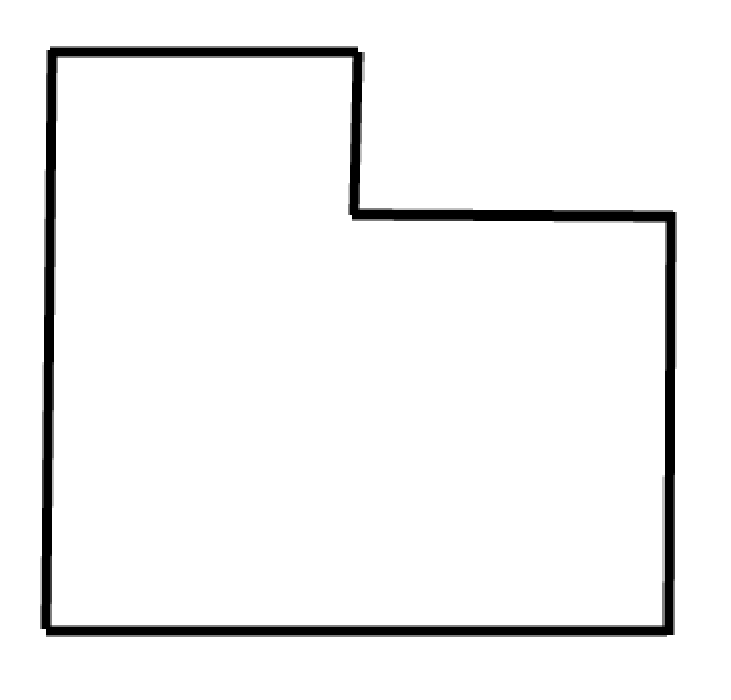
\includegraphics[scale=0.5]{figuras/exemplo_ambiente.eps}
		\caption[Exemplo de ambiente]{Exemplo de ambiente.}
		\label{img:exemplo_ambiente}
	\end{figure}

\section{Configuração e Integração das Tecnologias}

Nesta seção será apresentado o passo a passo para configuração e integração das tecnologias utilizadas durante este trabalho. A principal tecnologia utilizada é o pacote leJOS (Lego Java Operating System) NXJ, o qual possibilita a utilização da linguagem Java para implementação dos algoritmos durante a realização do trabalho. leJOS NXJ envolve um ambiente Java, um \textit{firmware} e uma API. 

O ambiente java disponibilizado pelo leJOS NXJ possibilita integração com a IDE Eclipse, facilitando o \textit{upload} de códigos, atualização de \textit{firmware} e utilização da API. O \textit{firmware} é necessário pois cria uma máquina virtual Java no NXT, possibilitando a execução de códigos Java no \textit{Brick}. E a API leJOS envolve uma variedade de classes e métodos com algoritmos já desenvolvidos e disponibilizados para utilização durante o desenvolvimento. Com a utilização da API, o desenvolvedor não se preocupa com a implementação de algoritmos comuns, como de navegação e obtenção de dados dos sensores.

A plataforma leJOS NXJ é multiplataforma, possibilitando sua utilização no \textit{Windows}, \textit{Linux} e \textit{MAC OS}, nas seções abaixo estão descritos os passos para instalação e configuração do leJOS NXJ nas três plataformas.

\subsection{Instalação no Windows} % (fold)
\label{sub:instalação_no_windows}
	
	Primeiramente, para possibilitar a comunicação entre o PC e o NXT, deve-se instalar um \textit{USB Driver}, o qual pode ser encontrado \href{https://www.lego.com/en-us/mindstorms/downloads}{aqui}, optando pela versão de seu Brick (no caso deste trabalho, o NXT). Após a instalação do USB Driver, deve-se instalar o JDK (Java Development Kit) versão 1.8, disponivel \href{http://www.oracle.com/technetwork/java/}{aqui}.

	Após a instalação do JDK, deve-se indicar as variáveis de ambiente do Java, adicionando o caminho do diretório do JDK instalado no \textit{PATH}. Para isso, siga os seguintes passos:

	\begin{enumerate}
		\item Clique em iniciar
		\item Painel de controle
		\item Sistema
		\item Configurações avançadas
		\item Clique na tab Avançado
		\item Variáveis de Ambiente
		\item Procure a variável JAVA\_HOME (Se não existir, crie uma)
		\item Edite a variável PATH e adicione o seguinte ao valor da mesma: \textit{$\%java\_home\% \textbackslash$ bin}
	\end{enumerate}

	Feito isto, basta testar se o Java está funcionando. Para isso, abra o \textit{Command Prompt} (CMD) e exeute o comando \textit{java}, caso esteja funcionando, será apresentado algumas opções de utilização do comando \textit{java}.

	Agora que o Java já se encontra instalado e funcionando, basta instalar o NXJ, o qual se encontra \href{http://www.lejos.org/}{aqui}. Baixe o arquivo \textit{Setup.exe}, execute o arquivo e siga os comandos de instalação apresentados pelo próprio instalador. Ao final da instalação, será executado um programa para \textit{upload} de um novo \textit{firmware} para o NXT. Feito isto, o leJOS já se encontra instalado e funcionando.
% subsection instalação_no_windows (end)

\subsection{Instalação no Linux} % (fold)
\label{sub:instalação_no_linux}
	
	Seguindo a mesma lógica de instalação apresentada na seção anterior, primeiramente deve-se instalar o USB Driver e o JDK. Por motivo de organização, apresenta-se primeiramente os passos de instalação do JDK, seguido do USB Driver.

	Para instalar o JDK, baixe a última versão do JDK disponível \href{http://www.oracle.com/technetwork/java/}{aqui}. Instale o JDK, de acordo com sua distribuição linux, e edite o PATH, adicionando o caminho do /bin do JDK instalado utilizando a variável \textit{$\%java\_home\% \textbackslash$ bin}. Para verificar se a instalação e configuração foram feitas corretamente, execute o comando \textit{java} no terminal e observe se informações de utilização do comando são apresentadas.

	Siga os seguintes passos para preparar e instalar o USB Driver:

	\begin{enumerate}
		\item Instale a lib \textit{libusb}, disponível \href{http://libusb.sourceforge.net}{aqui}, para que as ferramentas do leJOS possam acessar as portas USB do PC.
		\item  Tenha certeza que você possui acesso de leitura e escrita no dispositivo NXT USB. Para isso, verifique o arquivo /dev/bus/usb (especificidades em cada distribuição linux).
		\item Use regras Udev. Para isto, crie um arquivo chamado \textit{/etc/udev/rules.d/70-lego.rules} e adicione o seguinte conteúdo no mesmo:

		\begin{lstlisting}
			# Lego NXT brick in normal mode
			SUBSYSTEM=="usb", DRIVER=="usb",
			ATTRS{idVendor} == "0694",
			ATTRS{idProduct} == "0002", GROUP="lego",
			MODE = "0660"

			#Lego NXT brick in firmware update mode (Atmel SAM-BA mode)

			SUBSYSTEM == "usb", DRIVER == "usb",
			ATTRS{idVendor} == "03eb",
			ATTRS{idProduct} == "6124", GROUP="lego",
			MODE = "0660"
		\end{lstlisting}
	\end{enumerate}

	Feito isto, basta instalar o leJOS NXJ, de acordo com os passos a seguir:

	\begin{enumerate}
		\item Baixe o arquivo \textit{tar.gz} \href{www.lejos.org}{aqui}.
		\item Descompacte o arquivo no diretório \textit{/opt/lejos\_nxj/}.
		\item Crie a variável de ambiente \textit{NXJ\_HOME} apontando para o diretório onde foi descompactado o leJOS.
		\item Adicione o diretório \textit{/bin} da variável \textit{NXJ\_HOME} no seu \textit{PATH}.
		\item Caso tenha problema com permissões, deve alterar as permissões de execução neste diretório.
		\item Seu \textit{PATH} deve conter também o caminho para o binário \textit{ant}.
		\item Agora basta gerar a distribuição. Troque para o diretório de criação e rode \textit{ant}.
	\end{enumerate}

	Feito isto, basta atualizar o \textit{firmware} no seu NXT.
% subsection instalação_no_linux (end)



\section{Arquitetura da Solução}

\section{Considerações Parciais}